%Author - Akshay Vijayvergia
% $DA-IICT ID$ 201401061.


\documentclass[11pt]{article}

\oddsidemargin  -0.0in
\textwidth      6.5in
\headheight     0.0in
\topmargin      -0.25in
\textheight     9.0in
\parindent      0.0in
\parskip        0.05in

\usepackage{epsfig}
\usepackage{listings}

%used to include animation
\usepackage{animate}
\usepackage{animfp}

\begin{document}

% ---------------------------------------------------------------------------

\begin{center}
{\large SC462 Elements of Synthetic Biology: Life 2.0} \\
Prof. Manish K Gupta \\
DA-IICT\\
\bigskip
\hspace{0.25in} \\
{\Large\bf Cello: genetic circuit design automation} \\
Akshay Vijayvergia
\end{center}

% ---------------------------------------------------------------------------
\bigskip
\bigskip
\bigskip
\bigskip
\section*{Abstract}
DNA is the single most important part of all the organisms present on the planet. It consists of the genetic instructions used in the functioning, growth and development of all known living organisms. Due to this, to study biological architecture, we need to perform computations in living cells by DNA-encoded circuits which indeed process sensory information and control all the biological functions. But due to the various complexions like time and design, the computations become close to impossible. Thus to tackle this problem, we study Cello, which serves as a design environment where the user gives a verilog code as input that is automatically transformed into a DNA sequence providing a genetic circuit design. 

%%%%%%%%%%%%%%%%%%%%%

\bigskip
\section*{Introduction}

You could say "I want a cell that can detect arsenic, mercury, and cadmium in water and provide different color output signals. Also, those output signals should correlate to the concentration of metal detected." .These are the types of problems which could be efficiently simulated by Cello. Cello is a web based open source tool that is used to build genetic circuit diagrams. It's a joint initiative between Boston University and MIT, initiated by the CIDAR lab at Boston.

\bigskip

Its input consists of a Verilog script. This script is then parsed into a truth table which is further synthesised to generate a genetic circuit diagram with the genetically available gate types in the library. For simulating the circuit, a predicted score guides a breadth-first search, or a Monte Carlo simulated annealing search. Among all the predicted scores, the one with the highest score is selected. The one which is selected could then be implemented using the various genetic layouts. For finalising among one or more DNA sequences for the designated circuit, the Eugene language is used which further processes upon the rule based combinatorial design.

To briefly analyze Cello, firstly, we start with the actual/internal working of cello and begin to visualise how the verilog input is converted to a desired genomic circuit. Later we look into an example and find out the various functionalities provided by the web app.
%%%%%%%%%%%%%%%%%%%%%

\section*{Working}
\bigskip
\subsection*{VERILOG SPPECIFICATION}
When opening the website http://www.cellocad.org/verilog.html, we are greeted with a text editor which enables us to input the Verilog script. Cello accepts three forms of verilog scripts namely case statements, assign statements and structural statements. The verilog programs usually start with module keyword, followed by the name taking a list of output and input wire names as its arguments. We now focus on all the three specified verilog types.

\begin{enumerate}
\item Case: 
This style is usually preferred when we directly want to specify the truth table for our circuit.\bigskip
\begin{figure}[ht!]
\centering
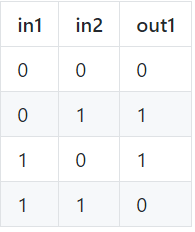
\includegraphics[width=4cm,height=12cm,keepaspectratio]{fig_1.png}
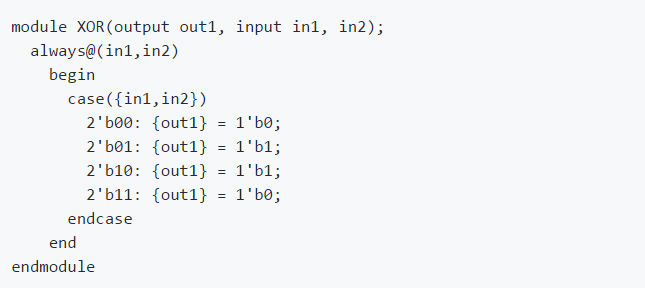
\includegraphics[width=11cm,height=14cm,keepaspectratio]{Screenshot_2.png}
\label{Case exmaple}
\end{figure}

\item Assign: 
This style is usually prefered when we want to specify circuit using boolean operators. For detailing the order of operations, parentheses are used. One thing should be noted that all the internal wires must be defined before use.\bigskip
\begin{figure}[ht!]
\centering
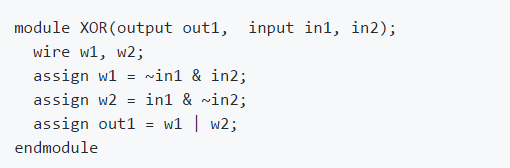
\includegraphics[width=11cm,height=14cm,keepaspectratio]{Screenshot_3.png}
\label{Assign exmaple}
\end{figure}

\item Structural: 
This style is usually prefered when we want  a gate-level wiring diagram to be specified. Again all the internal wires need to be defined before use.
\begin{figure}[ht!]
\centering
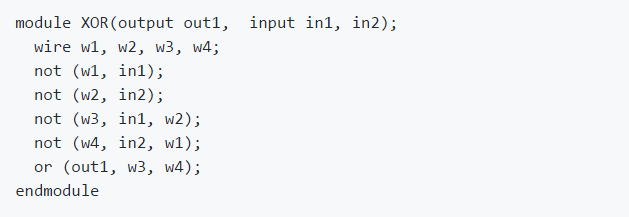
\includegraphics[width=11cm,height=14cm,keepaspectratio]{Screenshot_4.png}
\label{Structural exmaple}
\end{figure}

Here, within, the parenthesis, the first argument is the output wire and all the other trailing arguments are the inputs. The symbol at the beginning of each line is a operator.\\[\baselineskip]     
\bigskip
\bigskip
\bigskip
\bigskip
\end{enumerate}
By providing the verilog input in any of the above three designs, we then move onto the logical synthesis step.

\subsection*{LOGIC SYNTHESIS}
The verilog script is then parsed to generate a truth table. The truth table is then converted to the final wiring diagram in the following steps.
\begin{enumerate}
\item AND-Inverter Graph:
The table is converted to an AND-Inverted graph consisting of 2-input AND gates and NOT gates.
\item NOR-Inverter Graph:
The above is then converted to a NOR-Inverter Graph using DeMorgan's rule
\item Subcircuit substitutions:
The above is then simplified and further substituted with smaller but functionally equivalent logic diagrams in order to reduce the number of gates. In this step, other gate types can also be included.
\end{enumerate}
The above process is better described in the figure shown below: 
\begin{figure}[ht!]
\centering
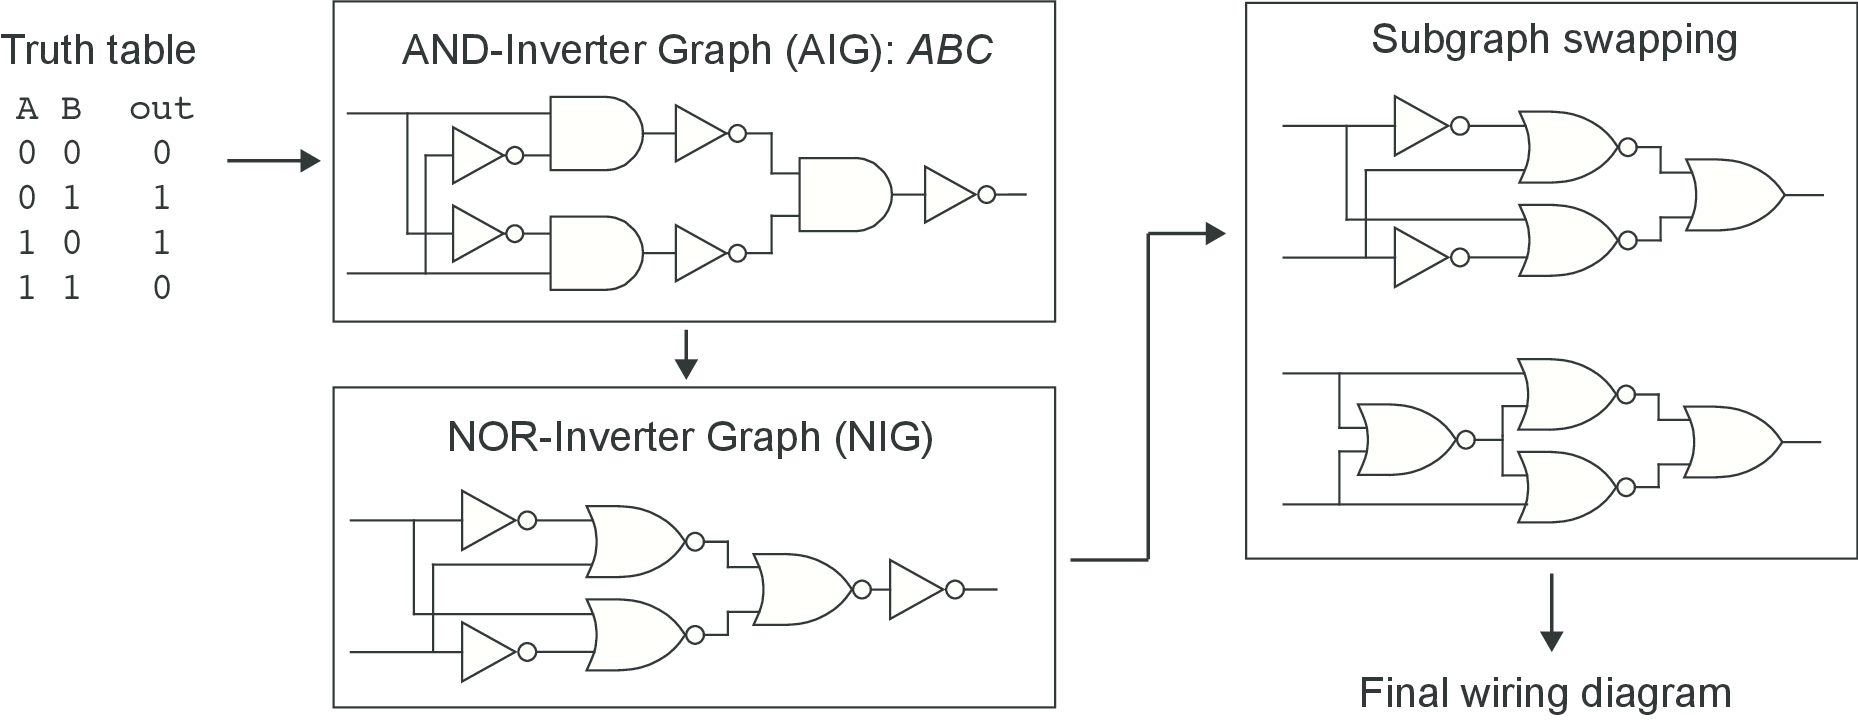
\includegraphics[width=18cm,height=18cm,keepaspectratio]{netsynth_xor_example.png}
\label{Case exmaple}
\end{figure}
\\[\baselineskip]    
After creating the simplified wiring diagram, we then assign gates to the diagram from the Cello library as per specification detailed in the next subsection.

\subsection*{GATE ASSIGNMENT}
Some basic gates in the gate library are shown below. If we want to add other gates to our library, we can add those using the UCF
\begin{figure}[ht!]
\centering
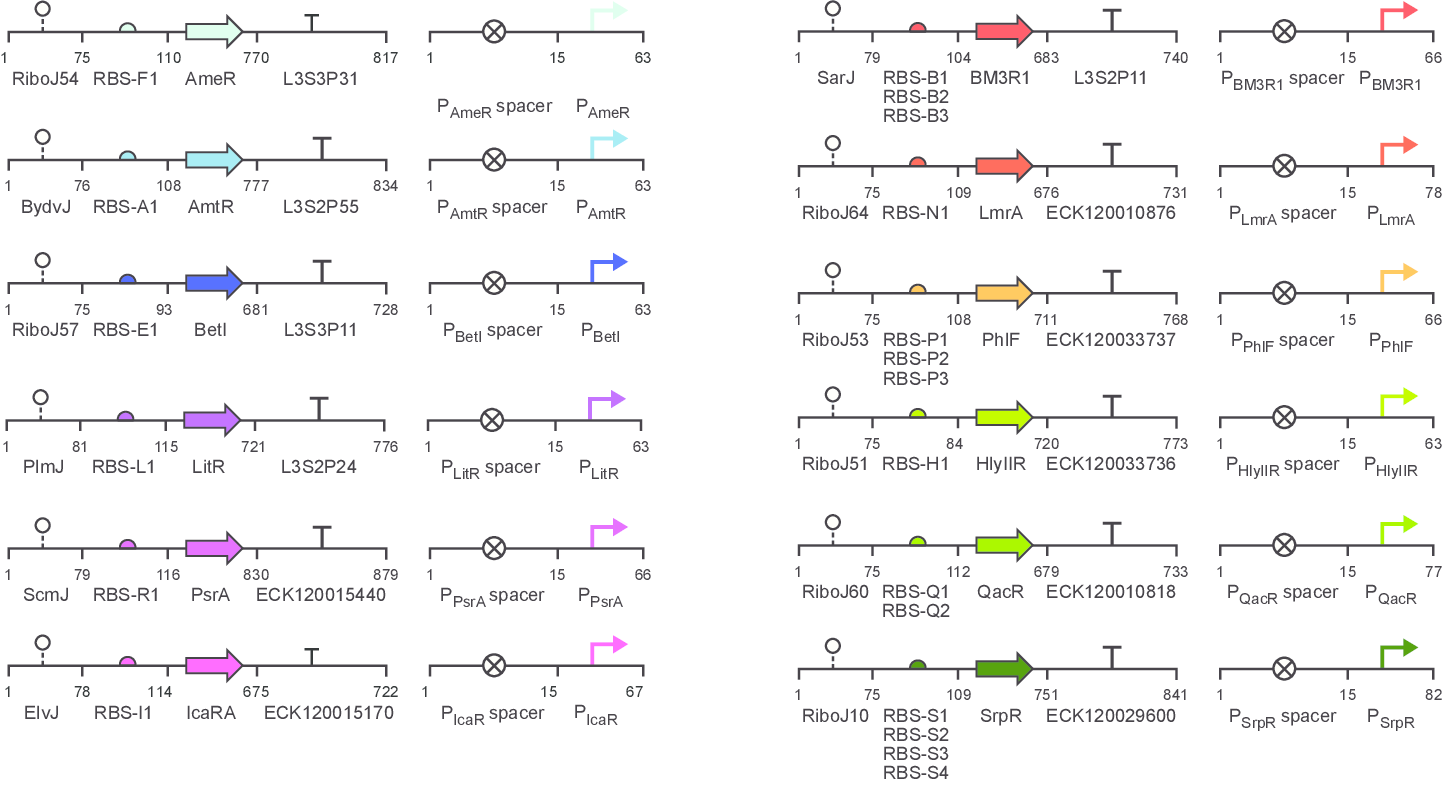
\includegraphics[width=16cm,height=16cm,keepaspectratio]{gate_parts_library.png}
\label{Case exmaple}
\end{figure}
\\[\baselineskip]    
All the gates shown above have an experimentally determined response function that relates one or more input values to an output value which is specified in standardized units (RPU = Relative Promoter Units). These response functions are then fitted to a Hill function which takes ymax, ymin, K,n as its 4 arguments.
The response functions of the above figured gates are shown below: 
\begin{figure}[ht!]
\centering
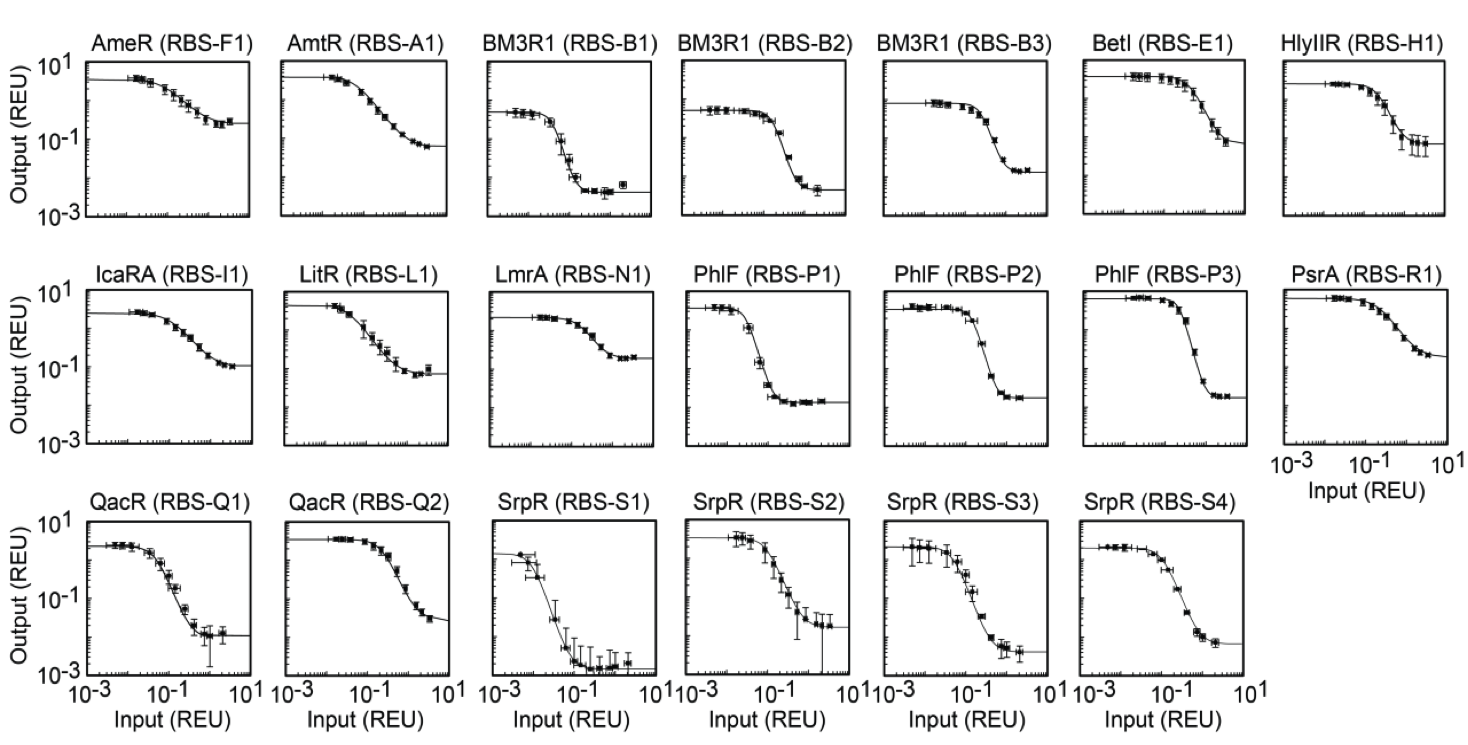
\includegraphics[width=16cm,height=17cm,keepaspectratio]{gate_response_functions.png}
\label{Case exmaple}
\end{figure}

But still, the main question remains as to how do we assign gates to all the elements in the circuit. This assignment is done using the following assignment algorithms.
\begin{enumerate}
\item Breadth-first search: 
This algorithm guarantees to select a genetic circuit with  a global max score among all other assignments. It starts with the gates which are closest to the inputs. The algorithm then goes one gate at a time where signal mismatches are faulty. For each acceptance in the traversal then next breadth first order gate is exhaustively assigned following the same procedure again until all the gates have been visited. After the completion, the circuit with the highest assignment score is selected.  
\item Hill climbing: 
This algorithm starts with a random assignment, and then swapping the assignment of 2 gates. Over here, gate 1 is randomly selected from the circuit to process and gate 2 is selected from the circuit or the gates which are left unused in the gate library for cello. The above specified swap is accepted if the initially initialized circuit score increases. After running this extensively on the whole circuit, the circuit with the highest assignment score is selected.
\item Simulated annealing: 
This is same as hill climbing except from the difference that the swaps that decrease circuit score with a probability that recombines/anneals over time are selected.
\end{enumerate}
Now for a given assignment, we can have a lot of combination of the arranging the genetic parts into physical diagrams. This problem is solved and assessed using the Eugene specification. The final DNA sequences that result from the Eugene variants is then placed into the genomic locations specified in the earlier describes UCF.   

\section*{Example}
Now let us take a verilog script and run it on cello webapp to find out the various logs and outputs provided by the software.
\begin{figure}[ht!]
\centering
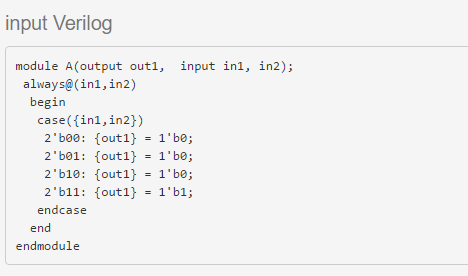
\includegraphics[width=10cm,height=11cm,keepaspectratio]{Screenshot_1.png}
\label{Case exmaple}
\end{figure}
\\[\baselineskip]    
On running the above case script for AND gate and selecting the inputs as pTac and pTet along with the output as RPF, we firstly get the following gate assignment after its logical synthesis as shown below:  
\begin{figure}[ht!]
\centering
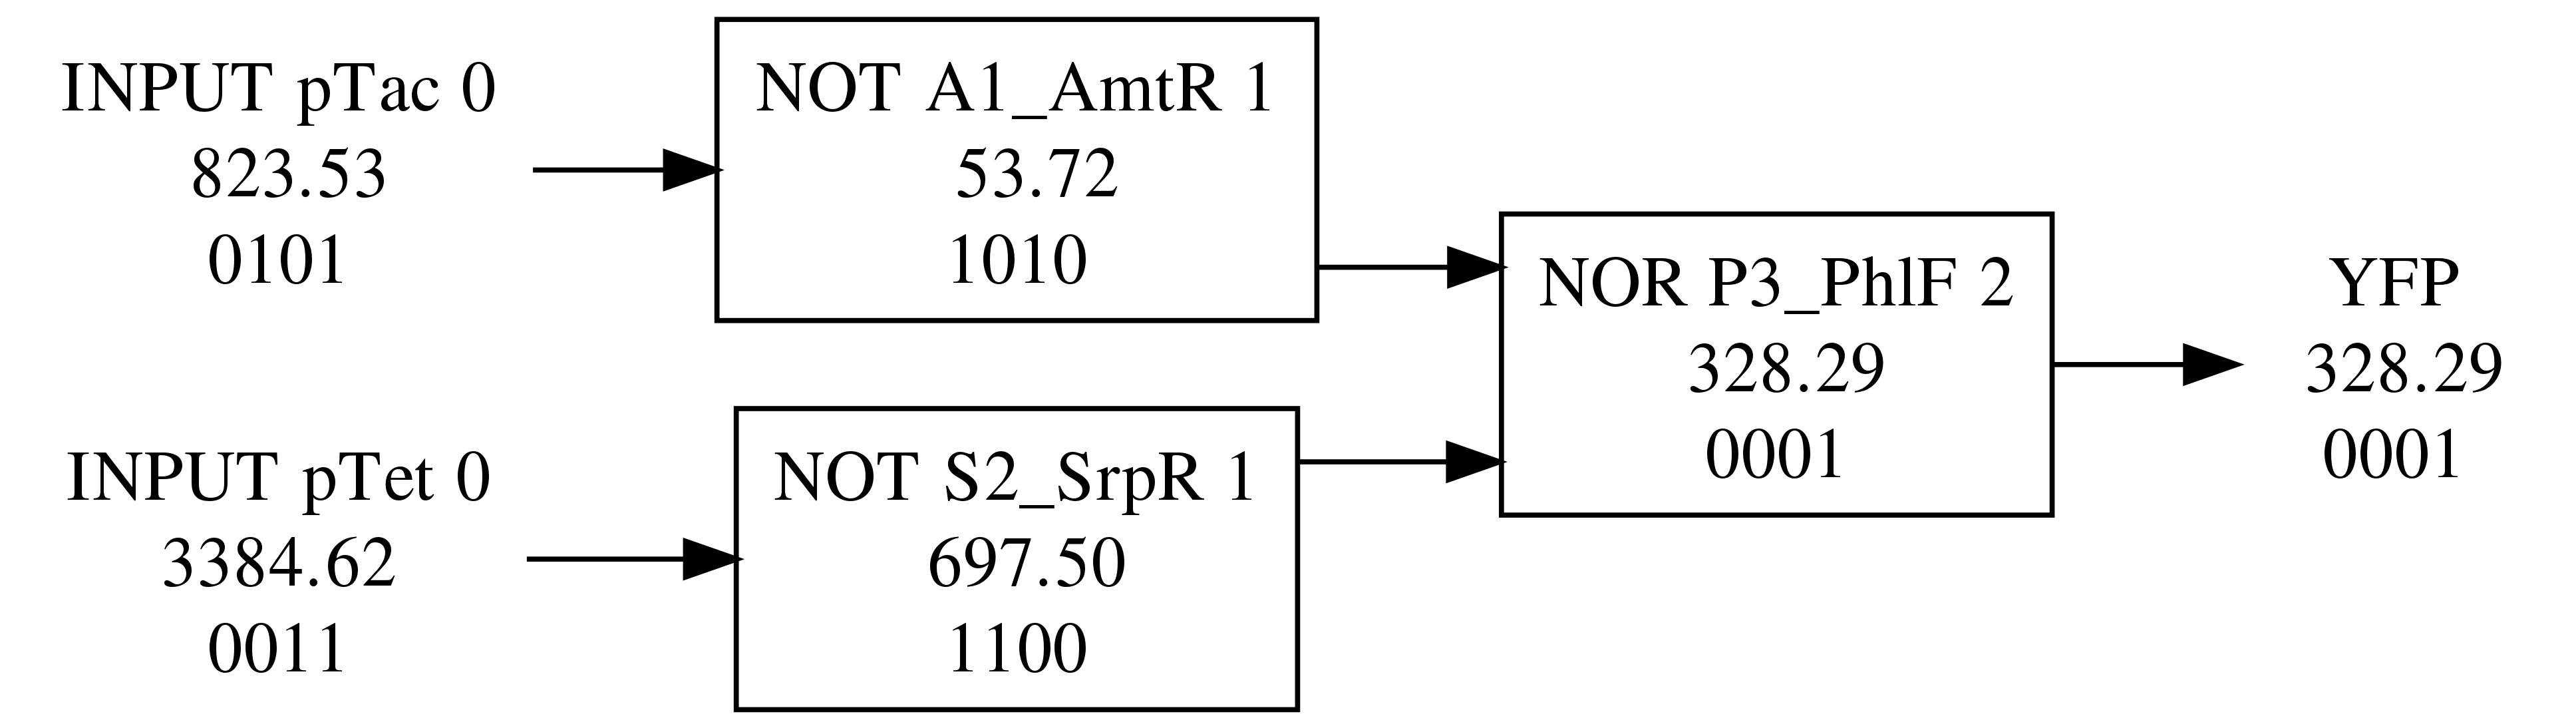
\includegraphics[width=16cm,height=16cm,keepaspectratio]{download.png}
\label{Case exmaple}
\end{figure}
\\[\baselineskip]   
\\[\baselineskip]   
\\[\baselineskip]   
\\[\baselineskip]   
The Response function of the above gate assignment circuit is shown below:
\\[\baselineskip]   
\begin{figure}[ht!]
\centering
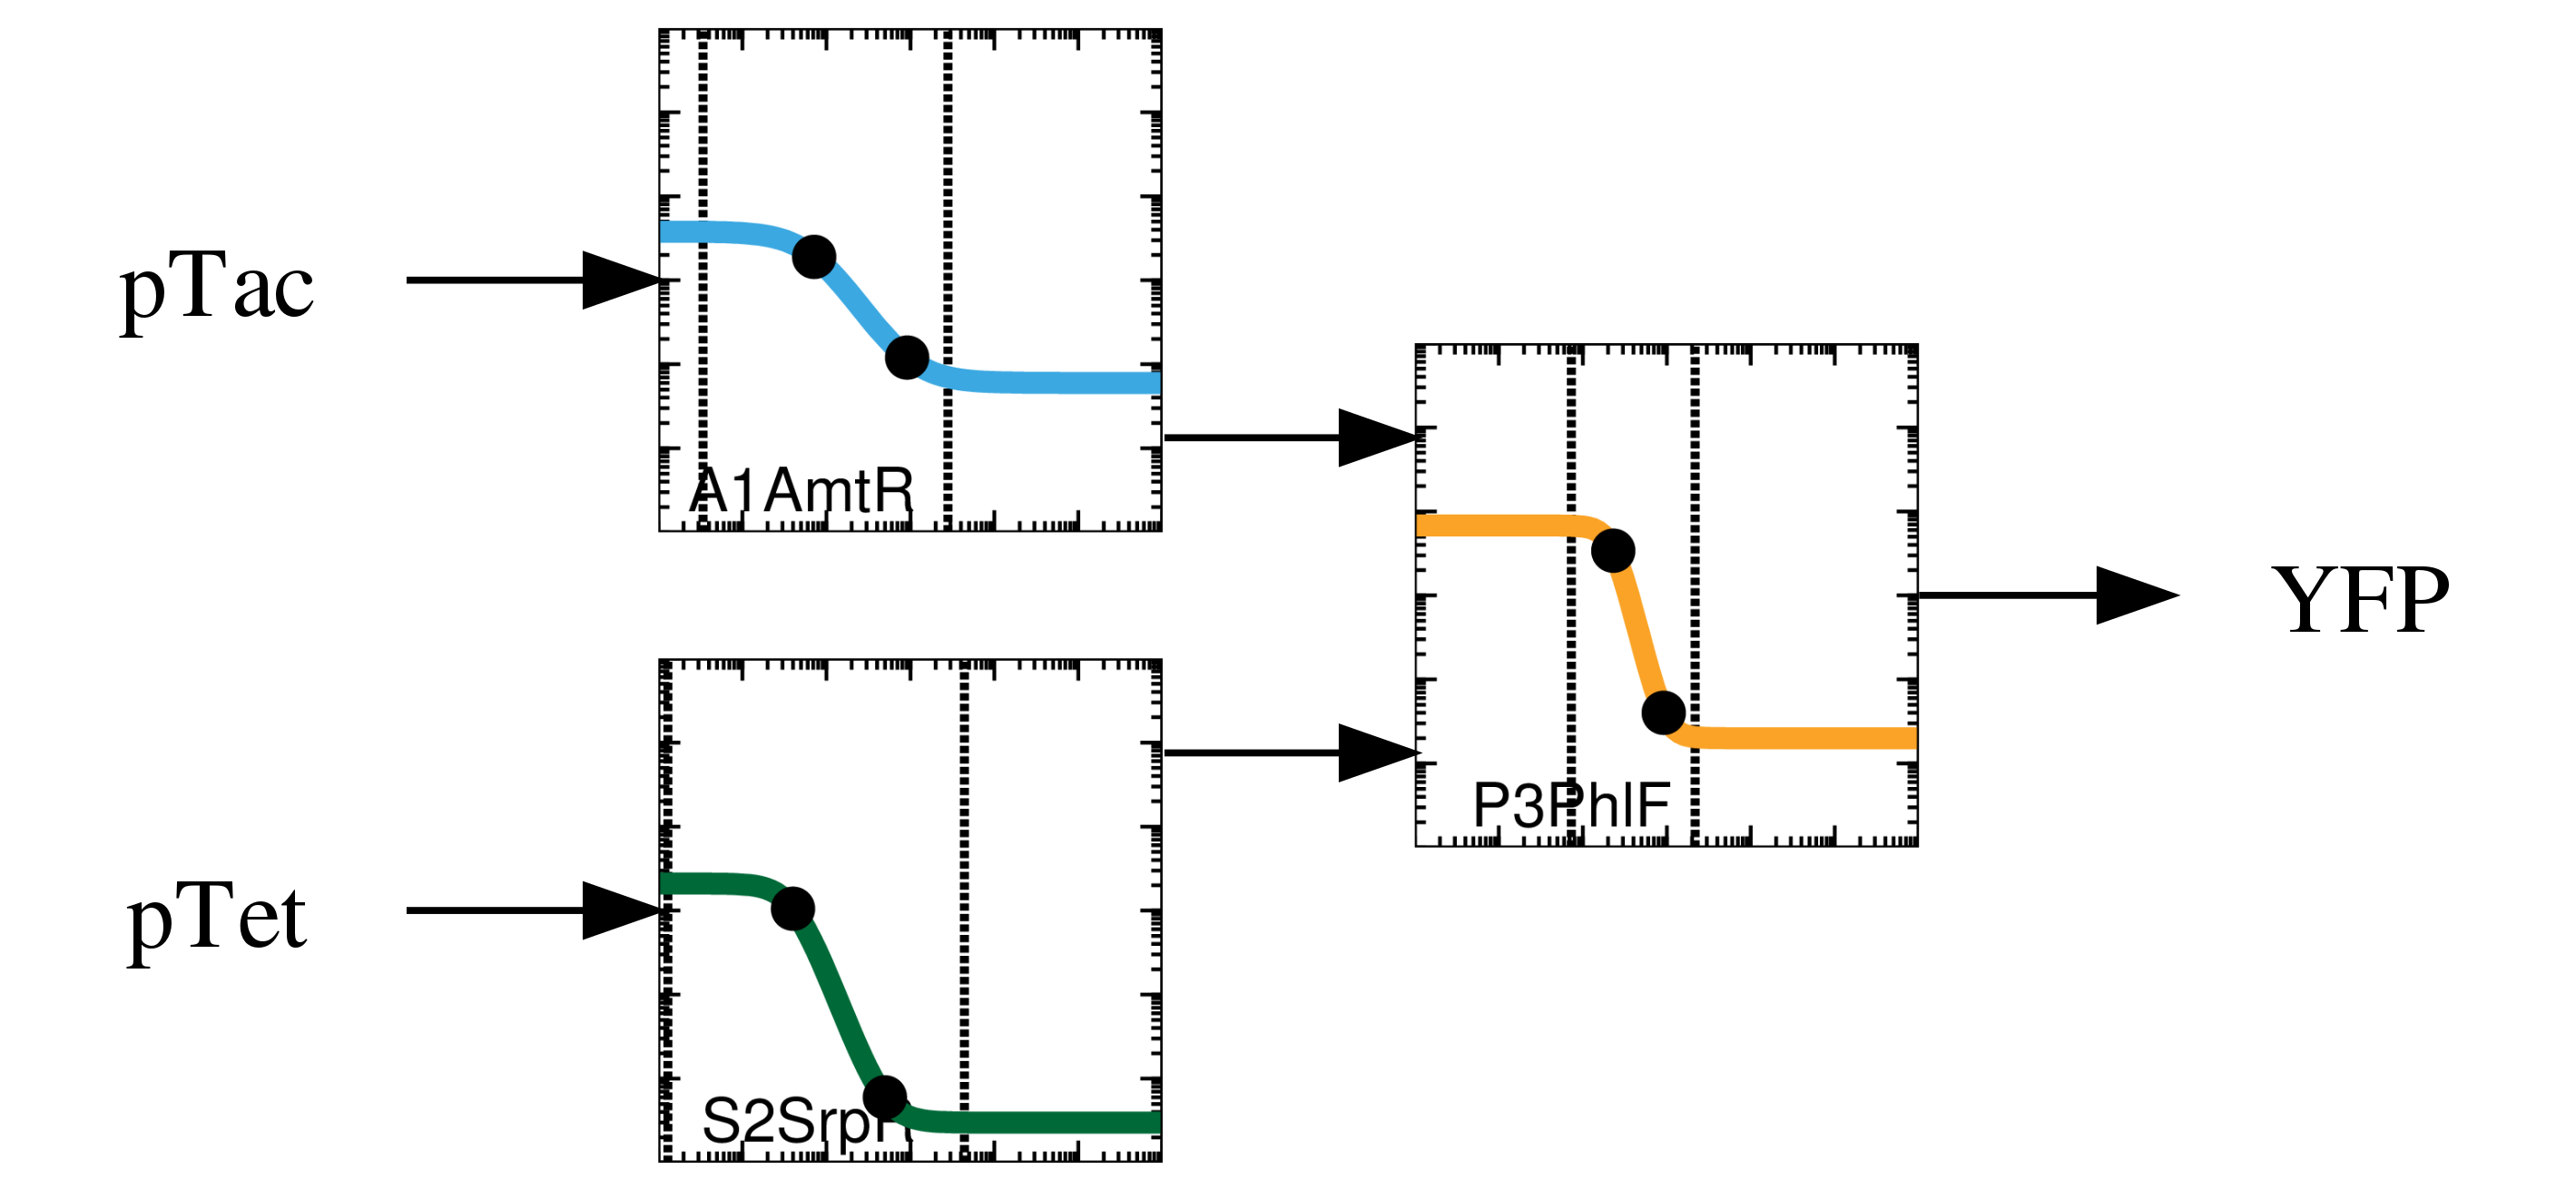
\includegraphics[width=16cm,height=16cm,keepaspectratio]{download (1).png}
\label{Case exmaple}
\end{figure}
\\[\baselineskip]   
As stated before, in the gate assignment subsection, all the gates have a  predefined output in RPUs(Relative Promoter Units). For the circuit, we see the predicted RPUs of the gates as shown below.
\begin{figure}[ht!]
\centering
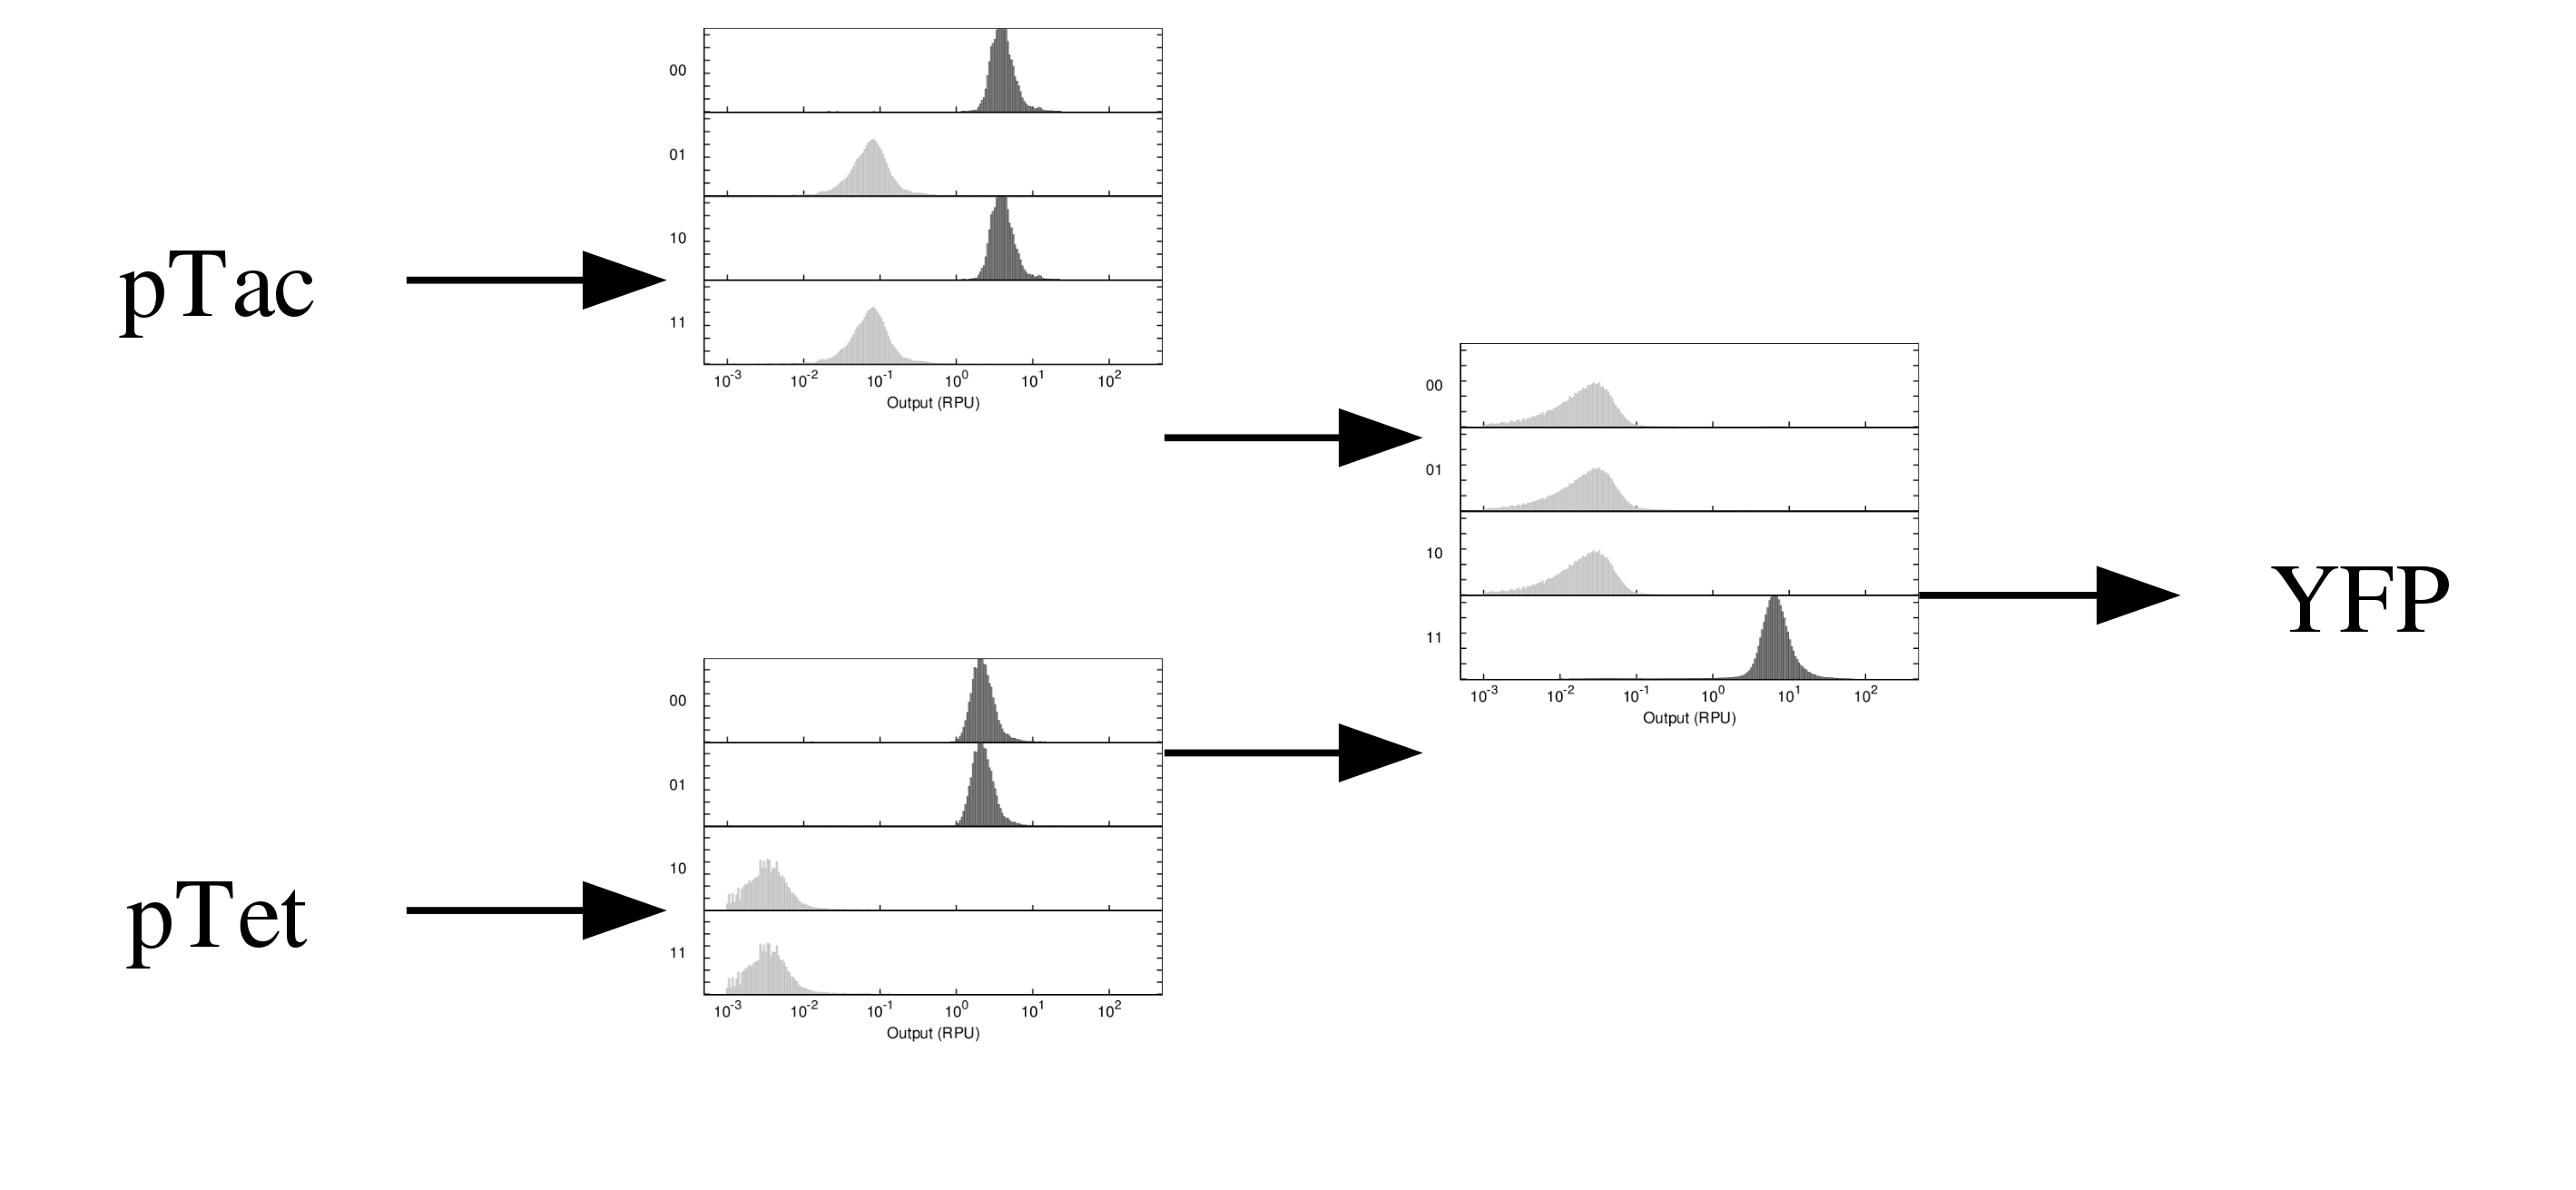
\includegraphics[width=16cm,height=16cm,keepaspectratio]{download (2).png}
\label{Case exmaple}
\end{figure}
\\[\baselineskip]   \\[\baselineskip]   \\[\baselineskip]   \\[\baselineskip]   
On providing the assignment algorithms we get the predicted gate output as shown below:
\begin{figure}[ht!]
\centering
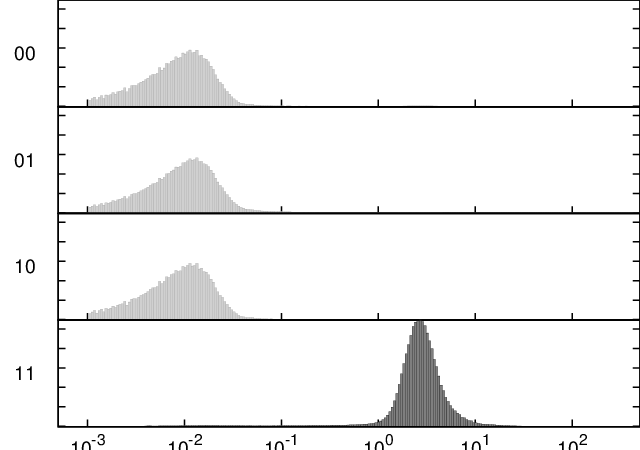
\includegraphics[width=12cm,height=12cm,keepaspectratio]{download (3).png}
\label{Case exmaple}
\end{figure}
\\[\baselineskip]   
The final circuit diagram created by the software is shown below after processing through the Eugene rules:
\begin{figure}[ht!]
\centering
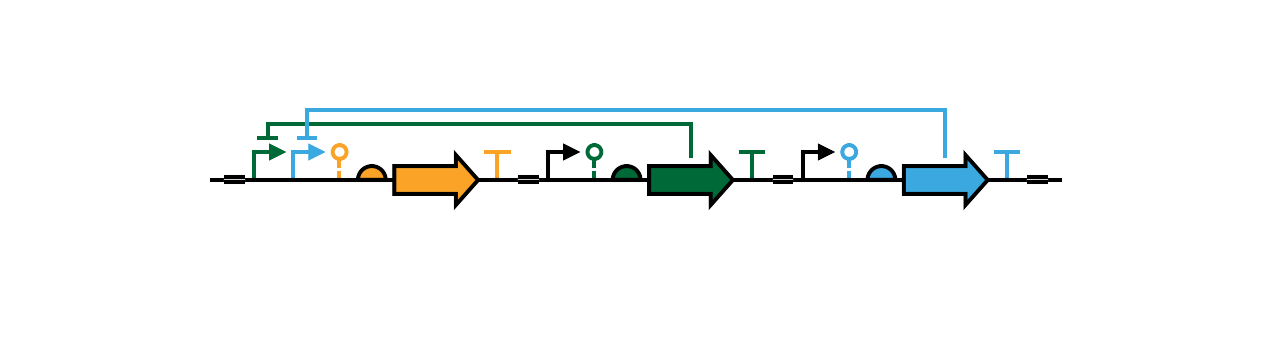
\includegraphics[width=12cm,height=12cm,keepaspectratio]{download (4).png}
\label{Case exmaple}
\end{figure}
In all the steps shown above, log files are also generated which further provide a detailed understanding of all the above steps as simulated by the Cello software. Finally, we are greeted with sbol_circuit, plasmid_circuit and plasmid_output log files which are indeed the results that we needed.


\end{document}